\chapter{Experiments and Results}
\label{chap:experiments}

% TODO maybe get rid of this section
\section{Problem Statement}
\label{sec:problem_statement}

In the Deep Q-Network section (\ref{sec:dqn})
I described an approach to deep reinforcement learning.
While the approach works well,
it has not managed to beat all games under consideration
nor would it generalize well to just any game
that fits the input description.
Much care has been taken to make DQN as generic as possible,
yet one detail stands out.

A single state consists of four consecutive image frames
in order to make the problem more Markovian,
a useful trait because it allows us to rely on
useful theoretical properties that have been established
for Markov settings.
However, not all games carry sufficient information
in the last four frames alone.
Some need a few more,
while others could conceivably
show information
that will then be needed to act correctly
after a long period of time has passed.
In other words, there could be hidden state
that the agent nevertheless had access to
at some point in the past.

\paragraph{}
My goal is now to explore different approaches
to this fixed-window history approach,
to explore different ways of dealing with time.
Ideally,
the learning technique should not employ an approach
that contains a fixed window anywhere at all.
However, such techniques are considered here as well.
% TODO discuss POMDP

\paragraph{}
The rest of this chapter is organized as follows.
First, I will examine the Arcade Learning Environment
in close detail in so far as this benefits
the following sections.
Then, I will closely investigate three approaches
to the time problem.
The three techniques discussed in this thesis are
\textit{Late Fusion},
\textit{3D Convolutions}
and \textit{LSTMs}.
Each in turn will be discussed,
then explored and evaluted.
Finally,
I will draw the conclusions of this thesis
in \ref{sec:conclusions}.

\section{Arcade Learning Environment}
\label{sec:arcade_learning_environment}
In order to fully understand the experiments that follow
and the implications of their results,
it is important to first have a closer
look at the Arcade Learning Environment
\parencite{bellemare13arcade}.
ALE is built on top of Stella
\footnote{http://stella.sourceforge.net},
an open-source Atari emulator.
It enables one to programmatically interact
with any compatible Atari game file.
This includes getting the screen in raw pixels,
access to the Atari's emulated RAM,
the game's current score
and actually interacting with the game by sending actions.

\paragraph{}
To appreciate the setting completely we will need to
investigate the hardware the games considered here used to run on.
The Atari 2600 was released in 1977.
Its CPU ran at 1.19 Mhz,
more than a 1000 times slower
than a single average core used for personal computers nowadays.
The size of the RAM was especially small compared to
what is used in modern days, with 128 bytes.

Of special interest to us is the console's graphic component.
The screen is 210 by 160 pixels
and could display up to 128 colors.

The Atari 2600 console is interacted with using
a joystick and a button.
The joystick can move in 8 directions.
Combining that,
along with pushing the button
while moving the joystick
(or not moving it)
gets us to 17 distinguishable actions.
Add one for not doing anything at all
and we have a total of 18 actions for our learning agent.

% TODO consider getting rid of this,
% just thought it was nice to see wtf it is
\begin{figure}[h]
\center
\begin{subfigure}[t]{.5\textwidth}
  \centering
  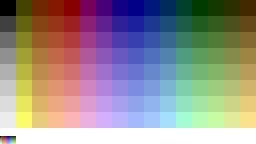
\includegraphics[width=\textwidth]{ntsc_palette.png}
  \vspace{.1\baselineskip}
  \caption{
    The Atari 2600 NTSC Palette used by many games.
    It allows 3 bytes for luminiscence
    and 4 bytes for chrominance,
    resulting in the 128 distinct colors
    you see here.
  }
  \label{fig:nips_network}
\end{subfigure}
\hfill
\begin{subfigure}[t]{.4\textwidth}
  \centering
  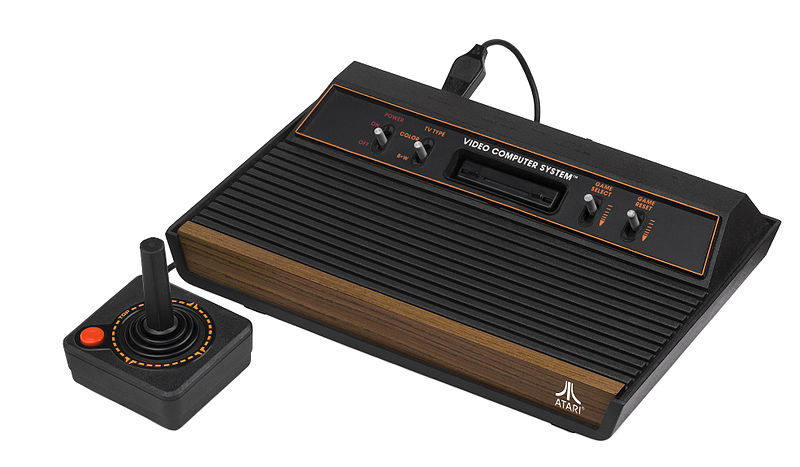
\includegraphics[width=\textwidth]{atari.jpg}
  \vspace{.1\baselineskip}
  \caption{
    The Atari 2600 with its joystick.
  }
  \label{fig:nature_network}
\end{subfigure}
\caption{}
\label{fig:dqn_networks}
\end{figure}

\subsection{Shortcomings}
\label{sub:shortcomings}
While the Atari's computational simplicity,
small screen
and relatively straightforward games
make it a great testbed for reinforcement learning,
the same characteristics
bring along a few shortcomings
that bear discussing.

\paragraph{}
First off, the Atari 2600
is entirely deterministic.
% TODO really want a ref on this
This allows some games to be abused
by learning how to exploit bugs
or otherwise causing situations
that would be very hard for a human to replicate,
yet that a learning algorithm could easily manage
in a deterministic setting.

This exploitation of a game's weak points
does not sound bad on its own
- after all, the agent is learning -
but it is obviously a case of overfitting
which should preferably be avoided.

% TODO should I mention in DQN?
DQN tries to avoid this by adding a random amount
of nullops at the start of the turn,
that is, the agent waits a random amount of turns
before it can play.

\paragraph{}
The console's determinism makes it so
that given the agent's history,
the next state given an action
can be known exactly.
However,
very few games actually need more than
a few frames of history
in order to achieve this Markov property.

Since the main interest of this thesis
is dealing with time,
long-term time dependencies would be especially interesting to investigate.
Sadly, however good of a testing environment ALE may seem,
it lacks thoroughly in this regard.
% TODO erase this if you don't
I will discuss later how to circumvent this lack of complexity partially.

\paragraph{}
% TODO(final) adjust if needed
I will now discuss two games in some detail
and shed light on their core distinctions
in order to later understand and explain
the differences between their learning results.

\subsection{Space Invaders}
\label{sub:space_invaders}

\subsection{Pong}
\label{sub:pong}

\subsection{General Setup}
\label{sub:general_setup}
All experiments that follow will be based on the DQN architecture
devised by \cite{Mnih2013}.





\section{Long Short-Term Memory Approach}
\label{sec:long_short_term_memory_approach}

\section{3D Convolutional Network Approach}
\label{sec:3d_convolutional_network_approach}

\section{Late Fusion Network Approach}
\label{sec:late_fusion_network_approach}

\section{Conclusions}
\label{sec:conclusions}


